\documentclass[onecolumn]{aastex63}
\usepackage{amsmath}
\usepackage{listings}

\lstset{frame=tb,
  language=Python,
  showstringspaces=false,
  columns=flexible,
  basicstyle={\small\ttfamily},
  commentstyle={\small\ttfamily},
  breaklines=true,
  breakatwhitespace=true,
  tabsize=4
}
\usepackage[T1]{fontenc}
\newcommand{\vdag}{(v)^\dagger}
\newcommand\aastex{AAS\TeX}
\newcommand\latex{La\TeX}
\shortauthors{McClellan}
\graphicspath{{./}{figures/}}
\begin{document}

\title{PhD Qualifying Examination \\ \small{\normalfont Literature Review and Research Overview}}
\author{B. Connor McClellan}
\affiliation{University of Virginia}
\keywords{}

\tableofcontents

\section{Literature Review}

\ifx
\subsection{Definitions}
%% What are things I learned in order to understand this paper?
\begin{itemize}
    \item \textbf{Resonance line radiation} refers to spectral lines caused by an electron jumping between the first excited state and the ground state of an atom or ion. The Lyman Alpha (Ly$\alpha$) resonance line is the $n=2\rightarrow1$ transition of hydrogen, and is one of the most common mechanisms by which astrophysical gas can cool \citep{neufeld1990}. Stellar Ly$\alpha$ radiation is frequently scattered by H atoms in the ground state within exoplanetary atmospheres.
    \item The \textbf{Poisson equation} is an equation of the form
    \begin{equation}
        \nabla^2 \phi = f
    \end{equation}
    It is a second-order differential equation which frequently comes up in electrostatics and fluid dynamics.
    \item An \textbf{eigenfunction expansion} is a method of solving differential equations, which utilizes a set of orthogonal eigenfunctions to construct solutions to said equations. As more eigenfunctions are included in the set, the solution converges closer to the true solution of the equation.
    \item A \textbf{line profile} is the shape of a spectral line on an intensity v. frequency plot. In our work we use a Voigt profile, which is the convolution of a Lorentzian (line wing) and a Gaussian (Doppler core) profile. For our purposes, we ignore the Doppler core contribution and use only the Lorentzian, since we care most about the solutions' behavior in the line wing.
\end{itemize}
\fi

\subsection{Scientific Purpose}
%% What is the science question addressed by the paper?
In this paper, it is shown that resonance-line radiation transfer in low-density, optically-thick media can be described by the Poisson equation. The equation is then solved using an eigenfunction expansion. The mean number of scatterings for escape are calculated, as well as the center and surface line profiles.

The optical depth is assumed to be so large that the transfer problem is dominated by the redistribution of radiation in the damping wings of the line. Modeling redistribution as a diffusion in frequency space naturally leads to a partial differential equation which turns out to be the Poisson equation. (Add more explanation about poisson) The resulting analytic solution is valid in the limit of large optical depth and is reported to match well with numerical results.

\subsection{Methods}
%% What is the method used to address the science question?
The physical setup of the problem is a uniform plane-parallel slab. The intensity is assumed to be nearly isotropic under the two-stream approximation (more specifically, what the author refers to as the ``Eddington approximation''). The derivation that follows relies upon the redistribution function and its expansion given by \cite{hummer1962} and \cite{1972ApJ...174..439A}, respectively. 

%\subsection{Derivations}
%%% Derivations of any critical equations that appear in the paper

Harrington's derivation begins with a second-order differential equation for the mean intensity.

\begin{equation} \label{harrington1}
    \frac{1}{3\phi^2(x)}\frac{d^2J(\tau, x)}{d\tau^2} = J(\tau, x) - (1-\epsilon)\int_{-\infty}^{\infty}J(\tau, x')q(x, x')dx' - \frac{G(\tau)}{4\pi}
\end{equation}

In order of appearance, the terms in this equation can be explained by their contributions to the behaviors of radiative transfer. $J(\tau, x)$ is a scattering sink term, and the integral is a source term which represents those photons which have scattered to a new frequency $x$ from a frequency $x'$. The $(1-\epsilon)$ factor in front of the integral represents the possibility of photon destruction through collisional de-excitation, and acts to reduce the number of photons produced by the source term it multiplies. $G(\tau)$ is a source term representing thermal emission, in units of radiation per unit area per unit mean optical depth. 

In the following steps of the derivation, Harrington reduces the problem to a Poisson equation by evaluating and expanding several of these terms. This is accomplished by 1) assuming that x is much larger than unity, meaning the frequencies in question are in the line wing, and 2) assuming that $|x'-x|$ is of order unity, meaning the frequency shift caused by redistribution is much smaller than the frequencies themselves. The following expansions are done in the limit of $|x-x'|$ being small. In Harrington's reasoning, this justifies the approximation of the line profile as a Lorentzian, which is accurate only in the line wing.

The general redistribution function within the integral, $q(x, x') = R_{II-A}(x, x')/\phi (x)$, is expanded according to \cite{1971JQSRT..11.1365A}. Notably, they define the integrated complementary error function as 

\begin{equation}
    \mathrm{ierfc}(z) \equiv \int_z^{\infty} \mathrm{erfc}(t) dt = \frac{1}{\sqrt{\pi}} e^{-z^2} - z\  \mathrm{erfc}(z)
\end{equation}

which Harrington incorrectly writes down as ``$i\ \mathrm{erfc(...)}$''. The first terms in the expansion are 

\begin{equation}
    R_{II-A}(x, x') \approx \frac{1}{2}\mathrm{erfc}(|r|+|s|) + \left(1 - \frac{a^2}{s^2} + \frac{a^4}{s^4}\right) \frac{a}{\pi s^2} \mathrm{ierfc}(|r|) + ...
\end{equation}

with $r=(x-x')/2$ and $s=(x+x')/2$. The first term in this expansion is ignored in the line wings, since it comes directly from the leading-order Gaussian term in the expansion of the Voigt profile. The next term of order $1/s^2$ is simply

\begin{equation}
    R_{II-A}(x, x') \approx \frac{a}{\pi s^2}\mathrm{ierfc}(|r|)
\end{equation}

By the same reasoning, the line profile $\phi$ can be approximated as $\phi(x) \approx a/(\pi x^2)$ in the line wing. Dividing the redistribution function by this approximate line profile yields 

\begin{equation}
    q(x, x') = \frac{x^2}{s^2} \mathrm{ierfc}(|r|) \approx \left(1+\frac{2r}{x}\right)\left(\frac{1}{\sqrt{\pi}}e^{-r^2} - |r|\ \mathrm{erfc}(|r|)\right)
\end{equation}

using the binomial approximation to obtain $x^2/s^2 = (r+s)^2/s^2 = (1+r/s)^2 \approx 1 + 2r/s \approx 1 + 2r/x$. The last step in this approximation comes from the understanding that as long as $|x-x'|\ll 1$, $s \approx x$ at second order.

The $J(x')$ term in the integral in Eq. \ref{harrington1} is then expanded in a Taylor series about $x$.

\begin{equation}
    J(x') \approx J(x) + \frac{dJ(x)}{dx}(x' - x) + \frac{1}{2}\frac{d^2J(x)}{dx^2}(x'-x)^2 + ...
\end{equation}

Changing variables to $r$, the integral becomes

\begin{equation}
    2 \int_{-\infty}^{\infty} \left(1+\frac{2r}{x}\right)\left(\frac{1}{\sqrt{\pi}}e^{-r^2} - |r|\ \mathrm{erfc}(|r|)\right)\left[J(x) - 2\frac{dJ(x)}{dx}r + 2\frac{d^2J(x)}{dx^2}r^2 + ...\right] dr
\end{equation}

where the minus sign introduced by the change of variables has been used to flip the bounds of integration, which would nominally go from $\infty$ to $-\infty$ under the variable $r$.

The various combinations of terms evaluate as the following:

\begin{itemize}
    \item $\int_{-\infty}^{\infty} e^{-r^2} dr = \sqrt{\pi}$
    \item $\int_{-\infty}^{\infty} r^{n} e^{-r^2} dr = 0$ for all odd powers $n$
    \item $\int_{-\infty}^{\infty} r^2 e^{-r^2} dr = \sqrt{\pi}/2$
    \item $\int_{-\infty}^{\infty} |r|\ \mathrm{erfc}(|r|)\ dr = 1/2$
    \item $\int_{-\infty}^{\infty} r^n |r|\ \mathrm{erfc}(|r|)\ dr = 0$ for all odd powers $n$
    \item $\int_{-\infty}^{\infty} r^2 |r|\ \mathrm{erfc}(|r|)\ dr = 3/8$
\end{itemize}

Therefore, collecting nonzero terms and evaluating the integral, we are left with

\begin{equation}
    \begin{split}
    \int_{-\infty}^{\infty}J(x')q(x, x') &= 2 \int_{-\infty}^{\infty}
    \frac{1}{\sqrt{\pi}}e^{-r^2}J(x) 
    + \frac{2}{\sqrt{\pi}}r^2e^{-r^2} \frac{d^2J(x)}{dx^2}
    - \frac{4}{x\sqrt{\pi}}r^2e^{-r^2} \frac{dJ(x)}{dx}\\
    &\hspace{1.5cm}- |r|\ \mathrm{erfc}(|r|)\ J(x)
    - 2r^2\ |r|\ \mathrm{erfc}(|r|)\ \frac{d^2J(x)}{dx^2} \\
    &\hspace{1.5cm}+ \frac{4}{x}r^2\ |r|\ \mathrm{erfc}(|r|)\ \frac{dJ(x)}{dx}
    dr\\ \\
    & = 2\left[J(x) + \frac{d^2J(x)}{dx^2} - \frac{2}{x}  \frac{dJ(x)}{dx} -\frac{1}{2}J(x) - \frac{3}{4} \frac{d^2J(x)}{dx^2} + \frac{3}{2x}\frac{dJ(x)}{dx}\right]\\
    & = J(x) - \frac{1}{x}\frac{dJ(x)}{dx} + \frac{1}{2}\frac{d^2J(x)}{dx^2}
   \end{split}
\end{equation}

The physical implications of each of these terms is illuminating to consider. The first, $J(x)$, is an emission term that will cleanly cancel with the corresponding absorption term in the transfer equation. The next term, $-\frac{1}{x}\frac{dJ(x)}{dx}$, determines the mean change in frequency per scattering. Since it varies inversely with $x$, it serves to trap the photons at line center. The closer the photon's frequency $x$ is to zero, the larger contribution this term will have and the harder it will be for the photon's to escape out of the line's core. The second term, $\frac{1}{2}\frac{d^2J(x)}{dx^2}$ gives rise to diffusion. The second derivative serves to make the photon increment its frequency, $x$, by 1 in either direction. The absence of any frequency term in front means this ``random walk'' behavior isn't affected by the strongly-peaked line profile. Together, the two terms act to randomly diffuse photons in frequency space, with a mean shift that tends toward line center.

Keeping up to second order terms, the integral is plugged in to the original differential equation, Eq. \ref{harrington1}. Introducing a suitable change of variables, we will see that the problem reduces to the Poisson equation. We will continue to use the optical depth $\tau$ to represent the spatial dimension, but will now use $\sigma$ to represent the photon frequency. $\sigma$ is defined as

\begin{equation}
    \sigma(x) = \int_0^x \sqrt{\frac{2}{3}}\frac{1}{\phi(x)}dx
\end{equation}

such that

\begin{equation}
    \frac{dx}{d\sigma} = \sqrt{\frac{3}{2}}\phi(x).
\end{equation}

Under this change of variables, a new approximation can be made at large $x$. In the line wings, $\phi \approx a/(\pi x^2)$ and $\sigma$ becomes

\begin{equation}
    \sigma(x) \approx \int_0^x \sqrt{\frac{2}{3}}\frac{\pi x^2}{a}dx = \sqrt{\frac{2}{3}} \frac{\pi}{a}\frac{x^3}{3}
\end{equation}

A convenient cancellation under this approximation turns the coefficient of some of the diffusion terms to zero, reducing the frequency dependence to a second derivative of $J$ with respect to $\sigma$. The transfer equation is now

\begin{equation}
    \frac{\partial^2J}{\partial \tau ^2} + \frac{\partial ^2 J}{\partial \sigma^2} = 3\phi^2 \left[\epsilon J - \frac{G}{4\pi}\right]
\end{equation}

Thus, we have our Poisson equation. The equation states plainly that the diffusion through both space and frequency are described by a sink of radiation caused by collisional de-excitation and a thermal source of radiation, which are both sensitively dependent on the strongly-peaked line profile. Harrington replaces the line profile by a delta function in $sigma$, normalizing it appropriately such that the equation left to solve is 

\begin{equation}
    \frac{\partial^2J}{\partial \tau ^2} + \frac{\partial ^2 J}{\partial \sigma^2} = \sqrt{6} \left[\epsilon J - \frac{G}{4\pi}\right]\delta(\sigma)
\end{equation}

Here, Harrington introduces a boundary condition based on the two-stream approximation. With regard to the physical setup of the problem, the boundaries are defined to be at optical depths $+B$ and $-B$ for a total optical thickness $2B$. The condition, $J=-2H$ at the upper boundary and $J=2H$ at the lower, relates the mean intensity to the flux at the surfaces under the assumption that there are no external sources of radiation. Using the definition that $H = -\frac{1}{3\phi}\frac{\partial J}{\partial \tau}$ we find

\begin{equation}
    \begin{split}
        J(B, \sigma) &= \pm 2 H(B, \sigma) \\
        J(B, \sigma) &= \mp \frac{2}{3\phi}\left(\frac{dJ}{d\tau}\right)_{\pm B} \\
        \left(\frac{dJ}{d\tau}\right)_{\pm B} &= \mp \frac{3}{2}\phi J(B, \sigma)
    \end{split}
\end{equation}

\subsection{Citeable Results}
%%% A list of citeable results in the paper
\begin{itemize}
    \item
\end{itemize}

\subsection{Discussion and Concerns}
%% Are there any red flags?

The accuracy of the solution put forth in this paper is limited by the treatment of the boundary conditions. In the eigenfunction expansion, the spatial and frequency components of the differential equation are separated, yet the spatial eigenvalues are defined as being explicitly frequency-dependent. The resulting solution for large optical depths would suggest the mean intensity at the boundary of the slab is zero, if not for the ansatz introduced to produce a finite, non-zero result. This treatment is plainly incorrect, and its effects on the calculated spectrum have not been quantified. It is for this reason that we compare Harrington's solution to numerical results, as discussed in Section \ref{researchoverview}. 

\subsection{Personal Relevance}
%%% Place the work into a familiar context. How is the discussion in the paper related to your own research interests and experience?

\subsection{Summary}
%%% Reread the abstract, and offer summarizing commentary.
% --------------------------- %
\newpage
\section{Research Overview} \label{researchoverview}

\subsection{Introduction}

 A central problem in the study of exoplanet atmospheres is how to treat radiation in optically thick environments, where light is scattered much more readily than it is transmitted. My work over the past year has found and tested analytic solutions of the radiative transfer equation for resonant scattering of Lyman-alpha (Ly$\alpha$) photons by dense gases. The results of this work will be used to create a scheme to accelerate the Monte Carlo transfer in regions of high optical depth. The impact of this project is that it will allow rapid hydrodynamic calculations of irradiated exoplanet atmospheres.

Observations by \textit{Hubble Space Telescope} have found deep Ly$\alpha$ transits by the exoplanets HD 209458b (Vidal-Madjar et al. 2003), HD 189733b (Lecavelier et al. 2012), and  GJ 436b (Ehrenreich et al. 2015), indicating the presence of large exospheric clouds produced by escaping hydrogen atoms. These clouds are thought to originate as winds driven from the planets by the intense host star radiation. Radiation forces due to the large opacity in the Ly$\alpha$ line are expected to have a large impact on the cloud's dynamics. Modeling the interplay between radiation and hydrodynamics in these atmospheric outflows is a difficult problem, as Monte Carlo simulations are inherently time-consuming and computationally expensive. In the much simpler problem of light from a central point-source escaping a sphere of uniform density, the mean number of scatterings for a single photon can reach $10^{7}$ or higher for large optical depths, requiring a significant time investment to calculate numerically. \textbf{This is why I have computed the frequency-dependent spectrum and escape time distribution of the emergent photons directly, saving hundreds of CPU-hours. This analytic distribution is sampled to calculate the mean intensity and flux at a fraction of the computational cost of traditional numerical methods.} I compare these new analytic solutions for photon escape time distributions to Monte Carlo simulations to establish their relative validity in the limit of large Ly$\alpha$ line-center optical depth. In simulation zones with large optical depth, millions of steps can be replaced by one ``superstep'', drawing from my tabulated distributions. Once the solution is confirmed to match the experimental results, this method will be applied to grid cells in a radiation-hydrodynamic simulation for comparison with a radiation magnetohydrodynamics (Rad-MHD) code. By obtaining the radiation pressure on each cell face, hydrodynamic forces can be calculated in each cell without the need to simulate comings and goings of individual photons.

\subsection{Methods}

As a first step, I wrote a Monte Carlo radiative transfer code in \texttt{FORTRAN} that tabulates escape times and angles of photons escaping from a sphere of uniform density. From these quantities, the outgoing flux and mean intensity at the surface of the sphere are easily calculated. In practice, a more sophisticated MCRT code written by Phil Arras is used to collect data for our escape time distributions. Separately, I wrote an analytic solver in Python that outputs the flux and mean intensity at all points within the sphere based on the radiative transfer solution. The solver operates in three main stages. First, I expand the spatial dependence of the transfer equation in terms of spherical Bessel functions, and separate the time dependence as a Fourier series. I use a set number of spatial eigenmodes $n$, photon frequencies $\sigma$, and oscillation frequencies $\omega$ to calculate Fourier coefficients $J(n, \sigma, \omega)$. Then, these Fourier coefficients are used to calculate the mean intensity $J$ and flux $H$ as a function of radius $r$, photon frequency $\sigma$, and time $t$. Finally, the flux at the surface of the sphere is evaluated to find the probability distribution of photon escape times.

Developing this solver was a key step in that it allowed for direct comparison between the analytic solutions and the Monte Carlo radiation transfer results. However, upon further analysis, it was found that our initial approach to finding numerical solutions was somewhat flawed. The problem is much better suited to an expansion using Laplace transforms, rather than Fourier transforms. With this approach, an imaginary frequency variable $s = i\omega$ is swept through to find resonant responses from the equation. When a resonance is detected, a refinement algorithm hones in on the peak and returns an eigenfrequency. A sum of eigenfunctions corresponding to these eigenfrequencies will return a solution for the mean intensity, which can be used to find the flux and consequently the wait time distribution for photons escaping the sphere.

The code that makes up the new analytic solver takes input parameters that determine the number of desired spatial and frequency eigenmodes. To determine where (and how) the result converges, I will increase the number of eigenmodes and characterize how the resulting wait time distributions are affected. Once the outputs have converged satisfactorily, I will have confirmed that the solver accurately represents the true analytic solution. To use the escape time distribution as a Monte Carlo accelerant, it must show a correctly-shaped rise and exponential falloff. I have isolated groups of photons from the Monte Carlo based on their escape frequencies as shown in Fig. \ref{mc_freqs}, and next I will compare the escape time distributions of these sub-populations against the analytic result.

\begin{figure}
    \centering
    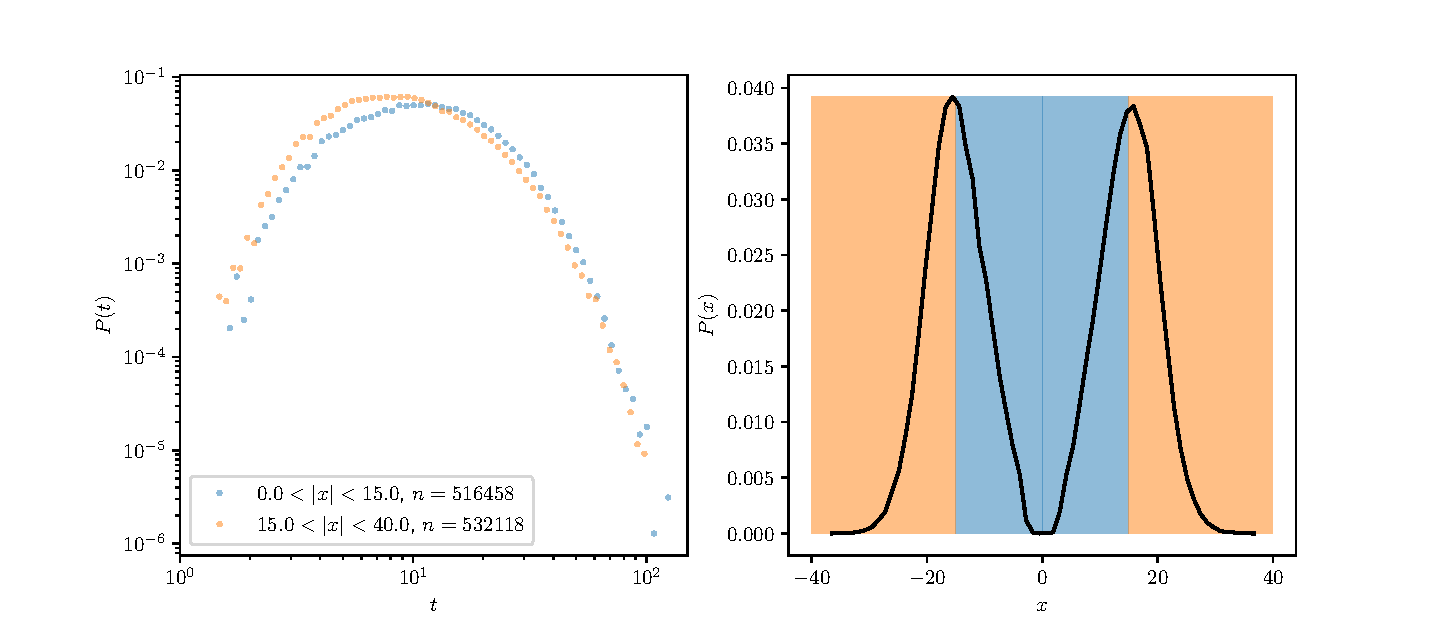
\includegraphics[width=\textwidth]{t-escape_frequency-study.pdf}
    \caption{Two frequency sub-populations identified in the Monte Carlo data with slightly different escape time distributions.}
    \label{mc_freqs}
\end{figure}

 These aims will quantify how well our analytic approach matches the equivalent numerical techniques, and their successful completion will form the basis for chapter 1 of my PhD thesis as a part of a broader effort to explore advanced numerical techniques in radiative transfer astrophysics. In follow-up work to be completed after my Master's defense, I will turn the results of this study into an acceleration scheme that will enable high-performance radiation hydrodynamics simulations of irradiated exoplanets. I anticipate that the method developed here may also be used in other contexts where Ly$\alpha$ transport is important, including emission from galaxies in the early universe.

\subsection{Results to Date}

Analytic groundwork was done to validate (or call into question) assumptions made in the theory papers preceding our work. In this section, these derivations are presented alongside numerical results to provide context and to illustrate the motivation for our more sophisticated analytic solution to this resonant scattering problem.

\subsubsection{Dimensional Scaling of the Time-Dependent Diffusion Equation}

The differential equation for time-dependent diffusion through the sphere is 
\begin{equation}
    -3 \frac{k\phi}{c} \frac{\partial J}{\partial t} + \nabla^2 J + \left( \frac{k}{\Delta} \right)^2 \frac{\partial^2 J}{\partial \sigma^2} = - \frac{\sqrt{6} kE}{4\pi \Delta^2} \delta(\vec{x}) \delta (\sigma - \sigma_s ) \delta (t)
        \label{timedependent}
\end{equation}

By replacing the differential operators with characteristic quantities and equating pairs of terms on the left-hand side of this equation, certain dimensionless scaling relations emerge. 

To find how the time-independent terms scale, I equate the second and third terms.

\begin{equation}
\begin{split}
    \frac{J}{R^2} &= \left(\frac{k}{\Delta}\right)^2 \frac{J}{\sigma_0^2}\\
    \sigma_0 &= \frac{kR}{\Delta}\\
    \frac{\sqrt{2\pi/27}}{a}x_0^3 &= kR \left(\frac{\sqrt{\pi}\tau_0}{kR}\right)\\
    x_0 &= \sqrt{\frac{27}{2}}\left(a\tau_0\right)^{1/3}
    \end{split}
\end{equation}

Thus, the theory predicts that the characteristic frequency in Doppler widths should scale as the cube root of the Voigt parameter $a$ multiplied by the line center optical depth $\tau_0$. I have tested our eigenmode solution against this scaling by computing an escape time distribution for $\tau_0 = 10^5, 10^6, 10^7$, and $10^8$. I use two different values as a ``characteristic frequency'' $x_0$. One is the inverse of the lowest-order imaginary eigenfrequency, which determines the late-time exponential falloff of the escape time distribution. The other is the value of $x$ at the peak of the escape time distribution. In Fig. \ref{tau_scaling}, the values of the characteristic frequency for each of these methods are plotted against the optical depth in the simulation. Overplotted is the line $x = \sqrt{27/2}\ (a\tau)^{1/3}$ for reference.

It can be seen that at lower optical depths, the power law is somewhat steeper with an index of ~$1/2$. However, at larger optical depths, the escape time distribution characteristic frequency converges to a power law scaling of $(a\tau)^{1/3}$. Thus, in optically thick media, the eigenmode expansion solution method appears to be consistent with the expected analytic power law. In future work, I will increase the number of spatial and frequency eigenmodes used to obtain the escape time distributions from which the characteristic frequencies were extracted. This will confirm whether or not our solution method has converged, and will establish a comparative connection between that convergence and the power law trend. Additionally, I will test the other scalings that can be obtained by equating the temporal term in Eq. \ref{timedependent} to each of the other terms.

\begin{figure}
    \centering
    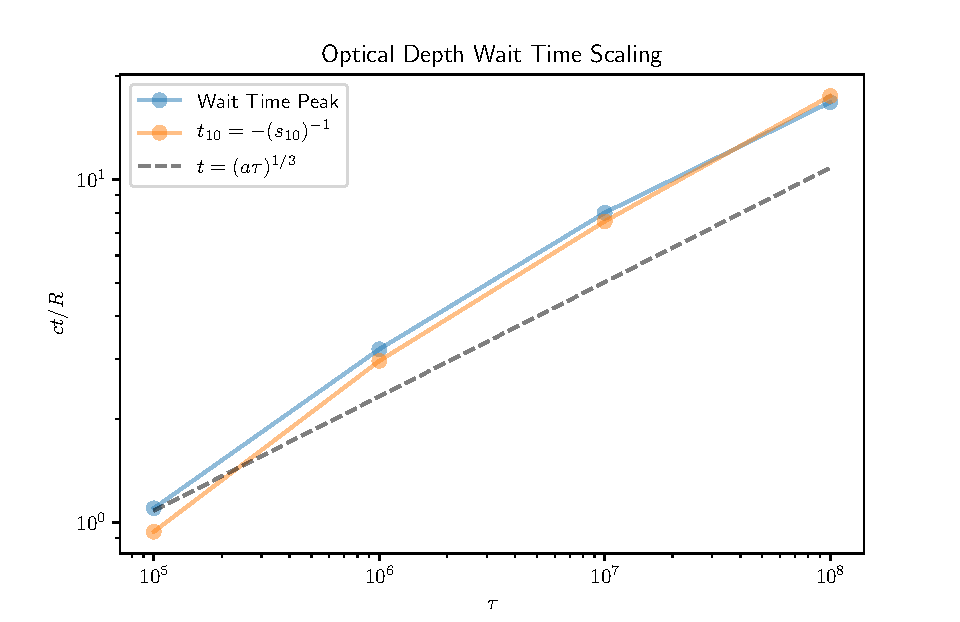
\includegraphics[width=\textwidth]{tau_scaling.pdf}
    \caption{Scaling of the characteristic frequency $x_0$ with the line-center optical depth, $\tau$. The escape time distributions were calculated with 6 spatial eigenmodes and 20 frequency eigenmodes.}
    \label{tau_scaling}
\end{figure}

\begin{equation}
    -3\frac{k\phi}{c}\frac{J}{t_0} = \frac{J}{R^2}
\end{equation}

\begin{equation}
    t_0 = \frac{-3R^2k\phi}{c}
\end{equation}


\subsubsection{Closed-Form Solutions for Ly$\alpha$ Resonant Scattering}

My aim in this section is to understand the internal consistency of the closed-form solution for Ly$\alpha$ resonant scattering proposed by \cite{2006ApJ...649...14D}, which is presented alongside our analytic and numerical results for quantitative comparison. The solution utilizes an eigenfunction expansion to separate the spatial and frequency variables; however, the spatial eigenvalues explicitly depend on the frequency. Thus, this expansion is not a true separation of variables. To assess the validity of their final result, I calculate the flux at the surface, $H$, starting from an earlier expression for the mean intensity before the approximation is made. This is then compared against their calculated mean intensity at the surface of the sphere using the two-stream approximation boundary condition.

In the two-stream approximation, it is assumed that the intensity is nearly isotropic---that is, it can be broken up into two components, $I_+(\tau)$ and $I_-(\tau)$. These will be referred to as the ``up'' and ``down'' intensities, respectively, and written shorthand as $I_+$ and $I_-$. The intensity is a function of the optical depth $\tau$ and angle $\mu = \cos{\theta}$, and is expressed in up and down components as

\begin{equation}
    I(\tau, \mu) = I_+ \delta(\mu - 1/\sqrt{3}) + I_- \delta(\mu + 1/\sqrt{3})
\end{equation}

The delta functions in angle are offset by $\pm 1/\sqrt{3}$, due to the normalization condition that the radiation pressure must be equal to $1/3$ the photon energy density. Under addition in quadrature, this condition is satisfied. The mean intensity is calculated as follows.

\begin{equation}
    \begin{split}
    J(\tau) &= \frac{1}{4\pi}\int d\Omega\ I(\tau, \mu)\\ 
    &= \frac{1}{2}\int_{-1}^1 d\mu\ I(\tau, \mu)\\
    &= \frac{1}{2}\int_{-1}^1 d\mu\ \left[I_+ \delta(\mu - 1/\sqrt{3}) + I_- \delta(\mu + 1/\sqrt{3})\right]\\
    &= \frac{I_+ + I_-}{2}
    \end{split}
\end{equation}

This makes intuitive sense; the mean intensity is the average of the ingoing and outgoing intensity. To calculate the flux, the intensity is integrated with an additional angular moment.


\begin{equation}
    \begin{split}
        H(\mu) &= \frac{1}{4\pi}\int d\Omega\ \mu\ I(\tau, \mu)\\
        &= \frac{1}{4\pi}\int_0^{2\pi} d\phi \int_0^1 d\mu\ \mu\ I(\tau, \mu)\\
        &= \frac{1}{2} \int_{-1}^1 d\mu\ \mu\ I(\tau, \mu)\\
        &= \frac{1}{2} \int_{-1}^1 d\mu\ \left[\mu I_+ \delta(\mu - 1/\sqrt{3}) + \mu I_- \delta(\mu + 1/\sqrt{3})\right]\\
        &= \frac{1}{2} \left( \frac{I_+}{\sqrt{3}} - \frac{I_-}{\sqrt{3}}\right) \\
        &= \frac{I_+ - I_-}{2\sqrt{3}}
    \end{split}
\end{equation}

Combining the flux, $H$, and mean intensity, $J$, we arrive at the following relations.

\begin{equation}
    \begin{split}
        &I_+ = J + \sqrt{3}H \\
        &I_- = J - \sqrt{3}H
    \end{split}
\end{equation}

To obtain a boundary condition that can be applied to our problem, we state that the incoming flux at the surface must be equal to zero, i.e. there is no external radiation. Therefore, at the surface, $I_- = 0$ and thus $J=\sqrt{3}H$. In the analysis that follows, I will demonstrate that the derivation in \cite{2006ApJ...649...14D} does not satisfy this surface boundary condition for the flux and mean intensity, and instead satisfies the condition $J = 2H$.

A few notational definitions must be made to relate various frequency and spatial variables. $x$, the distance from the source in Doppler widths, is related to the frequency variable $\sigma$ by 

\begin{equation} \label{sigma}
    \sigma = \frac{\sqrt{2\pi/27}}{a} x^3
\end{equation}

The Voigt function line profile is defined as 

\begin{equation} \label{lineprofile}
    \phi = \frac{a}{\sqrt{\pi} x^2}
\end{equation}

and

\begin{equation} \label{tau}
    R\kappa_0 = \tau_0
\end{equation}

Now, the result for the mean intensity from the end of \cite{2006ApJ...649...14D}'s derivation (Equation C17) reads

\begin{equation} \label{dijkstra}
    J(x) = \frac{\sqrt{\pi}}{\sqrt{24}a\tau_0}\left(\frac{x^2}{1 + \cosh{\sqrt{2\pi^3/27}(|x^3|/a\tau_0)}}\right)
\end{equation}

However, this has been multiplied through by $4\pi R^2$ to obtain the total emerging flux density at the surface. In our comparison, we wish to use the following expression instead.

\begin{equation} \label{c17/4piR^2}
    J(x) = \frac{1}{4\pi R^2}\frac{\sqrt{\pi}}{\sqrt{24}a\tau_0}\left(\frac{x^2}{1 + \cosh{\sqrt{2\pi^3/27}(|x^3|/a\tau_0)}}\right)
\end{equation}

This is checked against the boundary condition

\begin{equation} \label{bc}
    J = \sqrt{3} H
\end{equation}

by evaluating the surface flux derived from their Eq. C12. This equation reads 

\begin{equation} \label{c12}
    J(r, \sigma) = \frac{\sqrt{6}}{16 \pi^2 R} \frac{1}{rr_s} \sum_{n=1}^{\infty}\sin(\lambda_n r) \sin(\lambda_n r_s) \frac{\exp{(-\lambda_n |\sigma|/\kappa_0)}}{\lambda_n}
\end{equation}

Note that there is a typo in their equation, which I have resolved above. An extra factor of $\kappa_0$ appears in the numerator, which should have cancelled out in the previous step of their derivation. The quantity $\lambda_n$ is defined as 

\begin{equation} \label{lambdan}
    \lambda_n = \frac{n\pi}{R}
\end{equation}

at lowest order. Note that it is the second order term in the expansion of $\lambda_n$ that contains the line profile, which is frequency-dependent. To find the flux, we calculate the following derivative.

\begin{equation}
    \begin{split}
    H(r, \sigma) &= - \frac{1}{3\kappa_0 \phi}\frac{\partial J}{\partial r}\\
    &= - \frac{1}{3\kappa_0 \phi}\frac{\partial}{\partial r}\left(\frac{\sqrt{6}}{16 \pi^2 R} \frac{1}{rr_s} \sum_{n=1}^{\infty}\sin(\lambda_n r) \sin(\lambda_n r_s) \frac{\exp{(-\lambda_n |\sigma|/\kappa_0)}}{\lambda_n}\right)
    \end{split}
\end{equation}

Applying the product rule within the sum, we obtain

\begin{equation}
    H(r, \sigma) = - \frac{1}{3 \phi} \frac{\sqrt{6}}{16 \pi^2 R \kappa_0} \frac{1}{r_s} \sum_{n=1}^{\infty} \sin(\lambda_n r_s) \frac{\exp{(-\lambda_n |\sigma|/\kappa_0)}}{\lambda_n} \left[ \frac{-\sin(\lambda_n r)}{r^2} + \frac{\lambda_n \cos(\lambda_n r)}{r}\right]
\end{equation}

At this point, the expression is evaluated at the surface, $r=R$. Eq. \ref{lambdan} is substituted in for $\lambda_n$.

\begin{equation}
    H(\sigma) = - \frac{1}{3 \phi} \frac{\sqrt{6}}{16 \pi^2 R \kappa_0} \frac{1}{r_s} \sum_{n=1}^{\infty} \sin{\left(\frac{n\pi r_s}{R}\right)} \frac{\exp{(-n \pi |\sigma|/R\kappa_0)}}{\left(\frac{n\pi}{R}\right)} \left[ \frac{-\sin(n \pi)}{R^2} + \frac{n \pi \cos(n \pi)}{R^2}\right]
\end{equation}

The $\sin(n\pi)$ terms evaluate to zero, and the $\cos(n\pi)$ terms are equivalent to $(-1)^n$. We now have

\begin{equation}
    H(\sigma) = - \frac{1}{3 \phi} \frac{\sqrt{6}}{16 \pi^2 R^2 \kappa_0} \frac{1}{r_s} \sum_{n=1}^{\infty} (-1)^n \sin{\left(\frac{n\pi r_s}{R}\right)} \exp{(-n \pi |\sigma|/R\kappa_0)}
\end{equation}

Writing out the $\sin$ and $\exp$ terms, we are able to combine them into two separate factors raised to the power $n$, allowing the sum to be written as two geometric series.

\begin{equation}
    \sin{x} = \frac{e^{ix}-e^{-ix}}{2i}
\end{equation}

\begin{equation}
    \begin{split}
        H(\sigma) &= - \frac{1}{3 \phi} \frac{\sqrt{6}}{16 \pi^2 R^2 \kappa_0} \frac{1}{r_s} \sum_{n=1}^{\infty} (-1)^n \frac{\exp{(in\pi r_s / R)}-\exp{(-in\pi r_s/R})}{2i} \exp{(-n \pi |\sigma|/R\kappa_0)} \\
        &= - \frac{1}{3 \phi} \frac{\sqrt{6}}{32 i \pi^2 R^2 \kappa_0} \frac{1}{r_s} \sum_{n=1}^{\infty} (-1)^n \left[ \exp{\left(\frac{-\pi |\sigma|}{R\kappa_0} + \frac{i\pi r_s}{R}\right)^n}-\exp{\left(\frac{-\pi |\sigma|}{R\kappa_0} - \frac{i\pi r_s}{R}\right)^n}\right]
    \end{split}
\end{equation}

Using the geometric series

\begin{equation}
    \sum_{n=1}^{\infty}(-1)^nx^n = \frac{-x}{1+x}, \hspace{0.2cm} |x| < 1
\end{equation}

the sum can be evaluated to obtain

\begin{equation}
    H(\sigma) = - \frac{1}{3 \phi} \frac{\sqrt{6}}{32 i \pi^2 R^2 \kappa_0} \frac{1}{r_s} \left[\frac{-\exp{\left(\frac{-\pi |\sigma|}{R\kappa_0} + \frac{i\pi r_s}{R}\right)}}{1 + \exp{\left(\frac{-\pi |\sigma|}{R\kappa_0} + \frac{i\pi r_s}{R}\right)}}-\frac{-\exp{\left(\frac{-\pi |\sigma|}{R\kappa_0} - \frac{i\pi r_s}{R}\right)}}{1 + \exp{\left(\frac{-\pi |\sigma|}{R\kappa_0} - \frac{i\pi r_s}{R}\right)}}\right]
\end{equation}

Dividing top and bottom of each fraction through by its numerator, this simplifies to

\begin{equation} \label{before_trig}
    H(\sigma) = \frac{1}{3 \phi} \frac{\sqrt{6}}{32 i \pi^2 R^2 \kappa_0} \frac{1}{r_s} \left[\frac{1}{1 + \exp{\left(\frac{\pi |\sigma|}{R\kappa_0} - \frac{i\pi r_s}{R}\right)}}-\frac{1}{1 + \exp{\left(\frac{\pi |\sigma|}{R\kappa_0} + \frac{i\pi r_s}{R}\right)}}\right]
\end{equation}

Let us rewrite the terms in brackets as trigonometric functions, using the following variables as their arguments.

\begin{equation}
    \alpha = \frac{\pi |\sigma|}{R\kappa_0}; \hspace{0.4cm} \beta = \frac{\pi r_s}{R}
\end{equation}

\begin{equation}
    \begin{split}
    \frac{1}{1+e^{\alpha - i\beta}} - \frac{1}{1+e^{\alpha + i\beta}} &= \frac{1+e^{\alpha + i\beta} - 1 - e^{\alpha - i\beta}}{\left(1+e^{\alpha - i\beta}\right)\left(1+e^{\alpha + i\beta}\right)} \\
    &= \frac{e^{\alpha}\left(e^{i\beta} - e^{- i\beta}\right)}{\left(1+e^{\alpha - i\beta}\right)\left(1+e^{\alpha + i\beta}\right)} \\
    &= \frac{e^{\alpha}}{1 + e^{\alpha - i\beta} + e^{\alpha + i\beta} + e^{2\alpha}} 2i \sin{\beta} \\
    &= \frac{2i \sin{\beta}}{e^{i\beta} + e^{- i\beta} + e^{\alpha} + e^{-\alpha}} \\
    &= \frac{i \sin{\beta}}{\cos{\beta} + \cosh{\alpha}}
    \end{split}
\end{equation}

With this, Eq. \ref{before_trig} becomes

\begin{equation} \label{after_trig}
    H(\sigma) = \frac{1}{3 \phi} \frac{\sqrt{6}}{32 \pi^2 R^2 \kappa_0} \frac{1}{r_s} \left(\frac{\sin{\left(\frac{\pi r_s}{R}\right)}}{\cos{\left(\frac{\pi r_s}{R}\right)} + \cosh{\left(\frac{\pi |\sigma|}{R\kappa_0}\right)}}\right)
\end{equation}

We now take $r_s \rightarrow 0$, taking advantage of the approximation $\sin(x) \approx x$ for small $x$.

\begin{equation}
    H(\sigma) = \frac{1}{3 \phi} \frac{\sqrt{6}}{32 \pi R^3 \kappa_0} \left(\frac{1}{1 + \cosh{\left(\frac{\pi |\sigma|}{R\kappa_0}\right)}}\right)
\end{equation}

Substituting in Eq. \ref{sigma} for $\sigma$, Eq. \ref{lineprofile} for $\phi$, and Eq. \ref{tau} for $R \kappa_0$, we are left with

\begin{equation} \label{final}
    H(x) = \frac{1}{4\pi R^2}\frac{\sqrt{\pi}}{2\sqrt{24}a\tau_0} \left(\frac{x^2}{1 + \cosh{\left(\sqrt{2\pi^3/27}|x^3|/a\tau_0\right)}}\right)
\end{equation}

The two equations, Eq. \ref{final} and Eq. \ref{c17/4piR^2}, are related by the expression $J(x) = 2 H(x)$, suggesting that the two-stream boundary condition (Eq. \ref{bc}) is not satisfied. Instead of offsetting the angular delta functions by $1/\sqrt{3}$ to make the radiation pressure equal to one-third of the photon energy density, it is possible that Dijkstra used an offset of $1/2$. However, this yields an entirely different boundary condition, $J = 2H$, and does not properly normalize the radiation pressure.

\subsubsection{Analytic Solutions Compared with Monte Carlo}

\begin{figure}
    \centering
    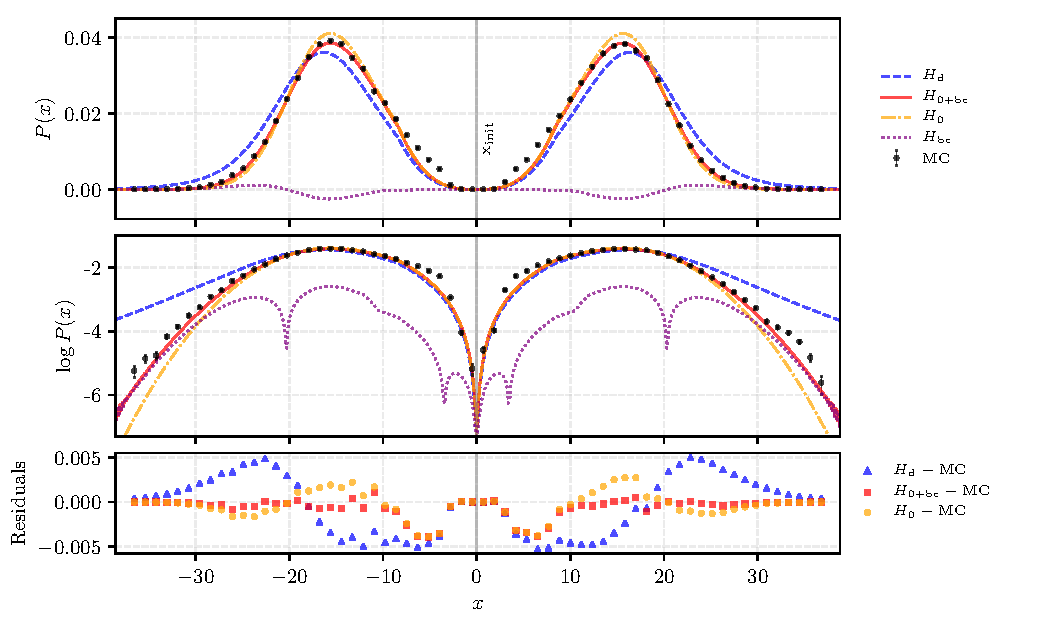
\includegraphics{pdf_xinit0.pdf}
    \caption{Analytic solution for the outgoing spectrum compared with Monte Carlo at a line center optical depth of $\tau_0 = 1 \times 10^7$. Photons are initialized with $\rm x = 0.0$. In the log-scale plot in the second panel, $|\rm H_{bc}|$ is shown instead of $\rm H_{bc}$.} 
    \label{fig:sol_mc_residual_0}
\end{figure}

\begin{figure}
    \centering
    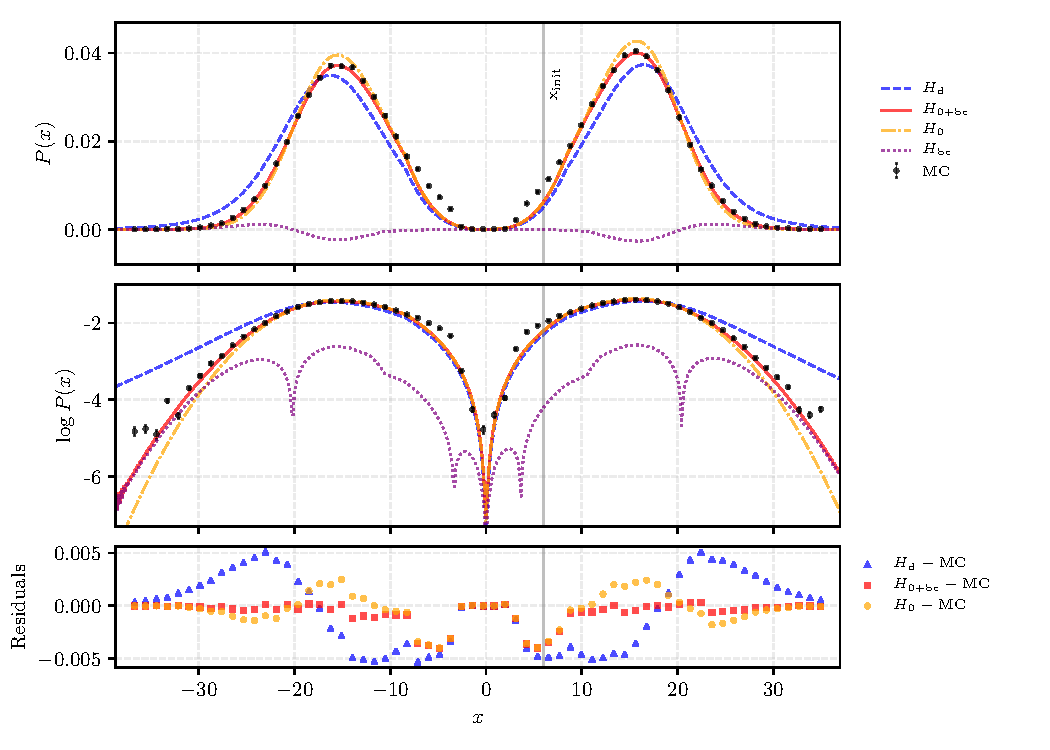
\includegraphics{pdf_xinit6.pdf}
    \caption{Analytic solution for the outgoing spectrum compared with Monte Carlo at a line center optical depth of $\tau_0 = 1 \times 10^7$. Photons are initialized with $\rm x = 6.0$. In the log-scale plot in the second panel, $|\rm H_{bc}|$ is shown instead of $\rm H_{bc}$.} 
    \label{fig:sol_mc_residual_6}
\end{figure}

\begin{figure}
    \centering
    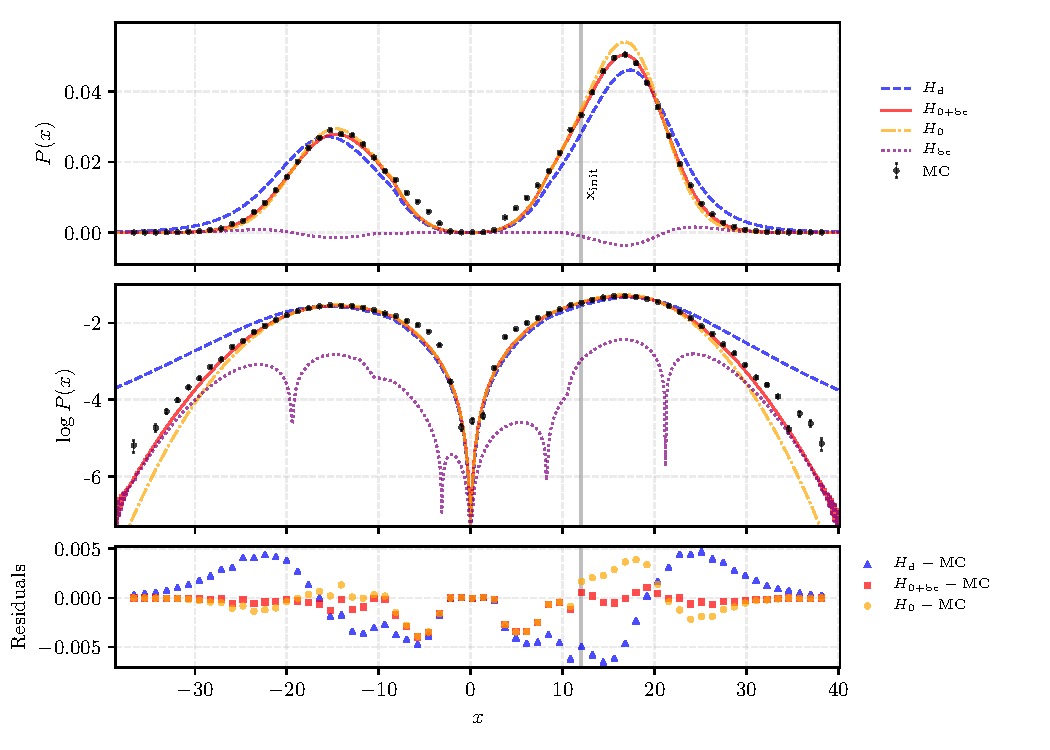
\includegraphics{pdf_xinit12.pdf}
    \caption{Analytic solution for the outgoing spectrum compared with Monte Carlo at a line center optical depth of $\tau_0 = 1 \times 10^7$. Photons are initialized with $\rm x = 12.0$. In the log-scale plot in the second panel, $|\rm H_{bc}|$ is shown instead of $\rm H_{bc}$.} 
    \label{fig:sol_mc_residual_12}
\end{figure}

One desired outcome of our work is to confirm that the analytic solution we present accurately characterizes the spectrum for the case where the monochromatic source of photons are not initialized with line-center frequencies. For each Monte Carlo dataset, the photons were initialized with a different starting frequency to evaluate the analytic solutions' accuracy with variation of the parameter $\rm \sigma_s$. This is related to the code parameter $\rm x_{init}$ by 
\begin{equation} \label{sigma0_xinit}
    \sigma_0 = \frac{\beta}{a} \rm x_{init}^3
\end{equation}

where $\beta = \sqrt{2 \pi / 27}$. Monte Carlo numerical simulations were performed with $\rm x_{init} = (0.0, 2.0, 4.0 ... 12.0)$ and optical depths $\tau_0 = (10^6, 10^7)$. In Fig. \ref{fig:sol_mc_residual_0}, \ref{fig:sol_mc_residual_6} and \ref{fig:sol_mc_residual_12}, these are compared with the analytic solutions at selected initial frequencies. In each of these figures, the contribution of the flux from our additive boundary condition correction, $H_{bc}$, is examined alongside the solutions $H_{\rm d}$ and $H_{\rm 0}$. The corrected solution, $H_{\rm 0 + bc} = H_{\rm 0} + H_{\rm bc}$, has considerably lower residuals to Monte Carlo than the other solutions, especially in the line wing. It is evident that the solution $H_{\rm d}$ derived by \citet{harrington1973} diverges significantly from the Monte Carlo simulations in the line wings. The $H_{\rm bc}$ correction term, when added to the solution $H_0$ derived by \citet{2006ApJ...649...14D}, produces a successful analytical result that characterizes the probability distribution of frequencies for escaping photons, including situations in which the photons are given initial frequencies outside of the line core.

This can best be seen by comparing the results shown in Fig. \ref{fig:sol_mc_residual_0} with those in Fig. \ref{fig:sol_mc_residual_12}. The $\rm H_{0+bc}$ analytic solution remains accurate in the line wing when photons are emitted away from line center, while the residuals of $\rm H_d$ and $\rm H_0$ become noticeably larger. It can be concluded that the $\rm H_{bc}$ correction term more accurately represents the additional flux from photons that escape without ever being scattered through the line core.

\subsection{Summary}

\subsection{Thesis Plan}

I will spend the next 2 years on this project, funded via a research grant by Phil Arras. During this time, the work I do on radiation transfer in exoplanet atmospheres will form the first few chapters of PhD thesis. When the project is neatly wrapped up at the end of the funding period, I will return to work on hydrodynamic calculations of Type II X-ray bursts.

Our paper, ``Resonant Scattering in a Uniform Sphere with Large Optical Depth'', will be published in February of 2021. This paper will introduce our semianalytic approach to accelerated Monte Carlo radiation transfer and compare its performance to previous solutions by \cite{harrington1973} and \cite{2006ApJ...649...14D}. 

In the Spring 2021 semester, I will work to produce a 1D calculation of the effects of irradiating an atmosphere, taking radiative and pressure forces into account. Having introduced an acceleration scheme for Monte Carlo radiative transfer, we can now simulate the thicker, deeper parts of the atmosphere where Ly$\alpha$ radiation might be able to break up molecules in an earth-like planet. This radiation could also cause excitation that could explain H-alpha and H-beta absorption in exoplanet atmospheres \citep{2017ApJ...851..150H}. Since much can be learned from extending the radiative transfer calculations to high densities, we can increase the value of our computation time by accelerating the Monte Carlo simulations at high optical depths.

This upcoming paper is exploring how we accelerate using analytic solutions. We realized we needed the mean intensity inside the grid to get the escape time distribution, so we did that. Goal is if we can finish this paper on the semianalytic stuff in the next months, we right away try to get the accelerated monte carlo code working. We want to then do 1D hydrodynamics and focus on the radiation pressure forces. We can do this analtically as well, which means we can check our MC accelerated numerical results against the 1D analytic result. By the end of this summer we will have this second paper out. 

Three years of funding during the academic year starts this coming year for the grant. This upcoming year is guaranteed because it's internal to UVa, but the other two years depend on getting extensions for the grant. It's important that we can show forward progress, which is why we want to publish two papers before the grant extension application is due. Now that I'm on board we're making all this progress, so we can justify the extension. If we have 1-2 papers by the following summer (2022), we will be in a good position to ask NASA for an extension. We would also like to publish 1-2 applications papers in the following year to justify even more funding for the 3rd year.

(When I finish my PhD, here is what I will have contributed to astronomy). We have pushed forward the study of exoplanetary research by calculating radiation forces, excitation, and heating of the upper atmospheres of exoplanets. We will apply these results for direct comparison with the aforementioned Hubble observations.

Don't need to say anything about grants, just say how long you're going to spend on it. 

\bibliography{bibliography}{}
\bibliographystyle{aasjournal}

\end{document}